
\section{Benchmark Evaluation}
\label{sec:micro}

In this section we evaluate the heterogeneous implementation of our 
interface using several small micro-benchmarks designed to illustrate
that our implementation approaches the underlying performance of the
hardware, and that the optimizations described in Section~\ref{sec:impl}
are important.  All exeperiments are run on the Keeneland
supercomputer\cite{Keeneland}.  Each Keeneland node is composed of
two Xeon 5660 CPUs, three Tesla M2090 GPUs, and 24 GB of DRAM.  Nodes
are connected by an Infiniband QDR interconnect.

\subsection{Event Latency and Throughput}
\label{subsec:eventmicro}
We implemented two micro-benchmarks for evaluating the performance of
events.  The first micro-benchmark tests the latency required to trigger
events both within a node and between nodes.  Processors are organized
into a ring and the first processor creates a user event and passes it
to the next processor.  The next processor creates a new event dependent
on the first, and passes the new event along. A long chain of dependent events 
is constructed.  The experiment measures the time from the triggering
of the first event to the triggering of the last event.  In the one node
configuration there is only one processor and all events are local to the
node.  In all other cases, there is only one processor per node which
guarantees that all event triggers result in an active message.  
Table~\ref{tab:eventlat} shows the results for both configurations.

\begin{table}
\begin{center}
{ \small
\begin{tabular}{m{2cm}|c|c|c|c|c}
Nodes & 1 & 2 & 4 & 8 & 16 \\ \hline
Mean Trigger Time ($\mu$s) & 0.329 & 3.259 & 3.799 & 3.862 & 4.013 \\
\end{tabular}
}
\end{center}
\vspace{-6mm}
\caption{Event Latency Results.\label{tab:eventlat}}
\vspace{-4mm}
\end{table}

In the single node case the latency of triggering an event is only 
329 nano-seconds.  For the multi-node cases, the triggering time is
between 3-4 micro-seconds which is the same as the cost of GASNet
active messages on Infiniband\cite{GASNET07}.  The gradual increase in latency with
node count is because each node must poll the Infiniband connection with all other nodes.
This demonstrates that the total cost of performing event triggers is in
the hardware and the underlying software stack.

Our second micro-benchmark for events measures the maximum throughput of event
triggers.  This benchmark creates {\em levels} of events where every event at a level
corresponds to a merge of all of the events at the previous level.  The benchmark is therefore
characterized by the number events at each level called the fan-in/out factor.  
The events at each level are evenly distributed between the processors in the machine.
In the case of an $n$-node experiment, only $n-1$ active messages will be required 
per event trigger because the event subscription mechanism described in 
Section~\ref{subsec:eventimpl}.  Figure~\ref{fig:eventthroo} shows the event triggering
throughput versus total nodes for a range of fan-in/out factors.

\begin{figure}
\begin{center}
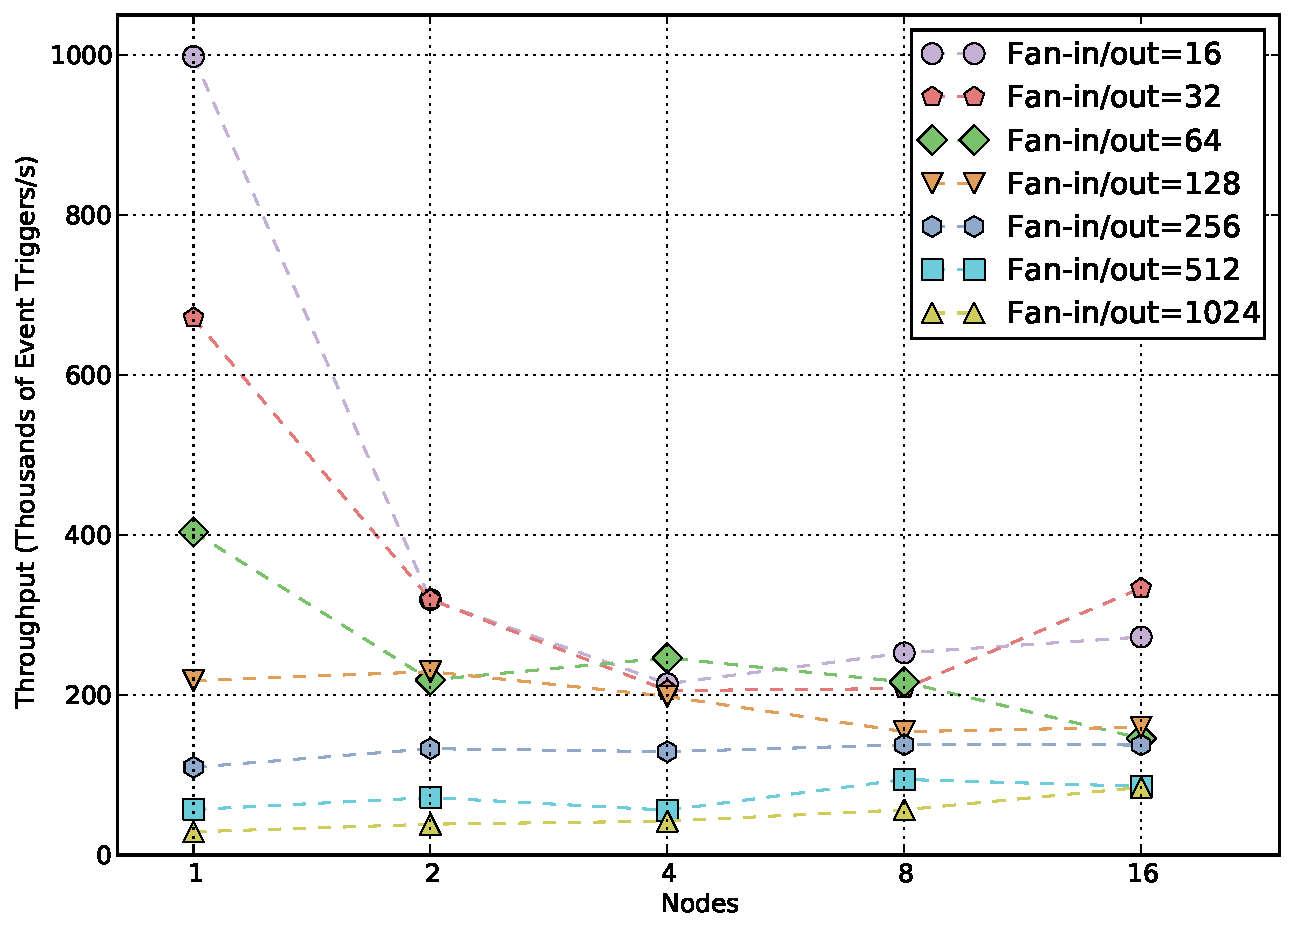
\includegraphics[scale=0.33]{figs/event_throughput.pdf}
\end{center}
\vspace{-6mm}
\caption{Event Throughput Micro-Benchmark.\label{fig:eventthroo}}
\vspace{-4mm}
\end{figure}

For small fan-in/out factors, throughput falls off initially going to two nodes as active
message become necessary, but starts increasing again at larger node counts.  Higher
fan-in/out factors require more messages and have lower throughput that increases with
node count.  In both cases the scaling of throughput is because the benchmark is
bound by the computational costs of active messages and not the bandwidth of the
interconnection network.  With more processors, more active messages can be processed
in parallel and performance improves.  
%Note we can further improve performance by increasing
%the number of threads per node for handling active messages (in these experiments there
%is one per node), but in real applications these threads would consume hardware cores and
%take away computational resources from the primary application.  This is only a viable
%option for memory or communication bound programs.  

The compute-bound nature of the benchmark demonstrate that active messages do not tax 
the interconnection network and leave bandwidth available for application data movement.  
The event throughputs sustained in this micro-benchmark are between one and two orders
of magnitude larger than the actual throughputs required by the real applications
described in Section~\ref{sec:apps}.

\subsection{Lock Throughput}
\label{subsec:lockmicro}
Our lock micro-benchmark is designed to measure the maximum throughput of lock
acquisitions.  The benchmark is characterized by the number of nodes, the number
of locks initially created by each node, and the number of {\em chains} of
lock requests per node.  A chain is 1024 lock acquire and release operations that
are serialized by event dependences.  Each node creates the specified number of locks and
informs all other nodes of its lock handles.  All nodes create the specified number
of chains by randomly selecting from the set of all locks in the system.  All chains
are predicated on a user event.  The experiment measures the time from the start of
the user event to the completion of all chains.

Figure~\ref{fig:fixedlock} shows the lock grant throughput versus nodes in the system
for a fixed number of total chains in the system (256 total).  Each line corresponds
to a number of locks per node.  At larger node counts there will be more total locks
in the system.  At small node counts, small numbers of locks per node cause high
contention and lock unfairness allows for very high throughput as many requests are
handled locally before locks are migrated.  Large values have more total locks which
results in lower contention and lower throughput because more lock migrations are
required per satisfied request.  At larger node counts, there are enough locks
in the system to remove contention and throughput increases.

\begin{figure}
\begin{center}
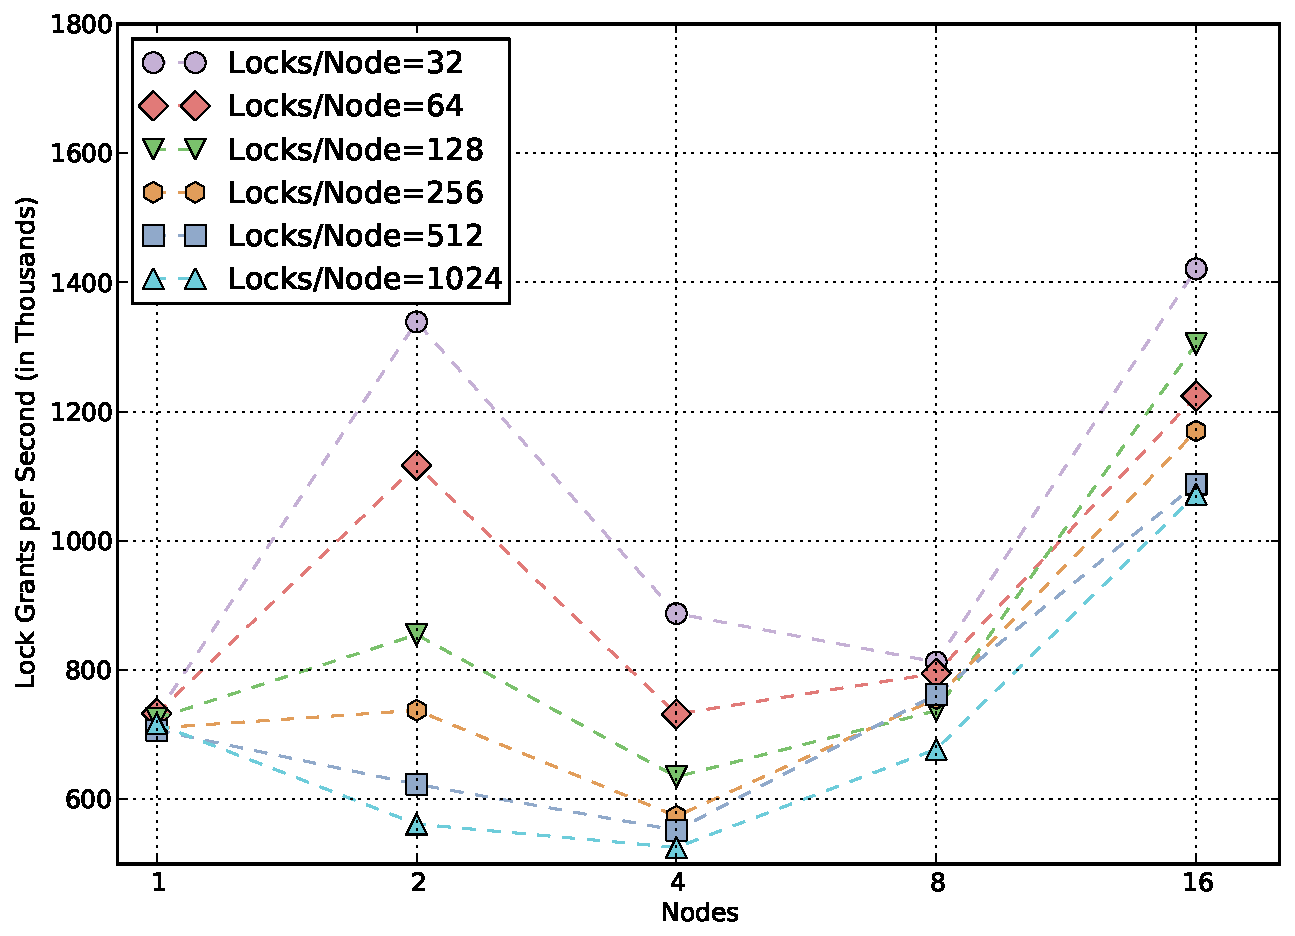
\includegraphics[scale=0.33]{figs/fixed_lock_chains.pdf}
\end{center}
\vspace{-6mm}
\caption{Lock Benchmark for Fixed Total Chains.\label{fig:fixedlock}}
\vspace{-4mm}
\end{figure}

To demonstrate that lock unfairness is also beneficial at larger node counts we show an alternative
cut of the experiment space.  In this case we fix the node count at 16 and plot
grant throughput as a function of chains per node for many different locks per node (also
total nodes in the system since node count is fixed).
The results can be seen in Figure~\ref{fig:fixednode}.  At very small chains per node
there is little contention and throughput is high.  At larger chains per node there is
more contention for locks and throughput drops because of higher lock migrations.  Note that 
as soon as chains per node is greater than total locks, the expected number of users per lock 
per node becomes more than one.  It is exactly at this point on each line that throughput
begins to improve again!  This is because as soon as there are multiple expected users on
a node, the unfairness property of the lock can amortize the cost of lock migration which
yields better throughput.

\begin{figure}
\begin{center}
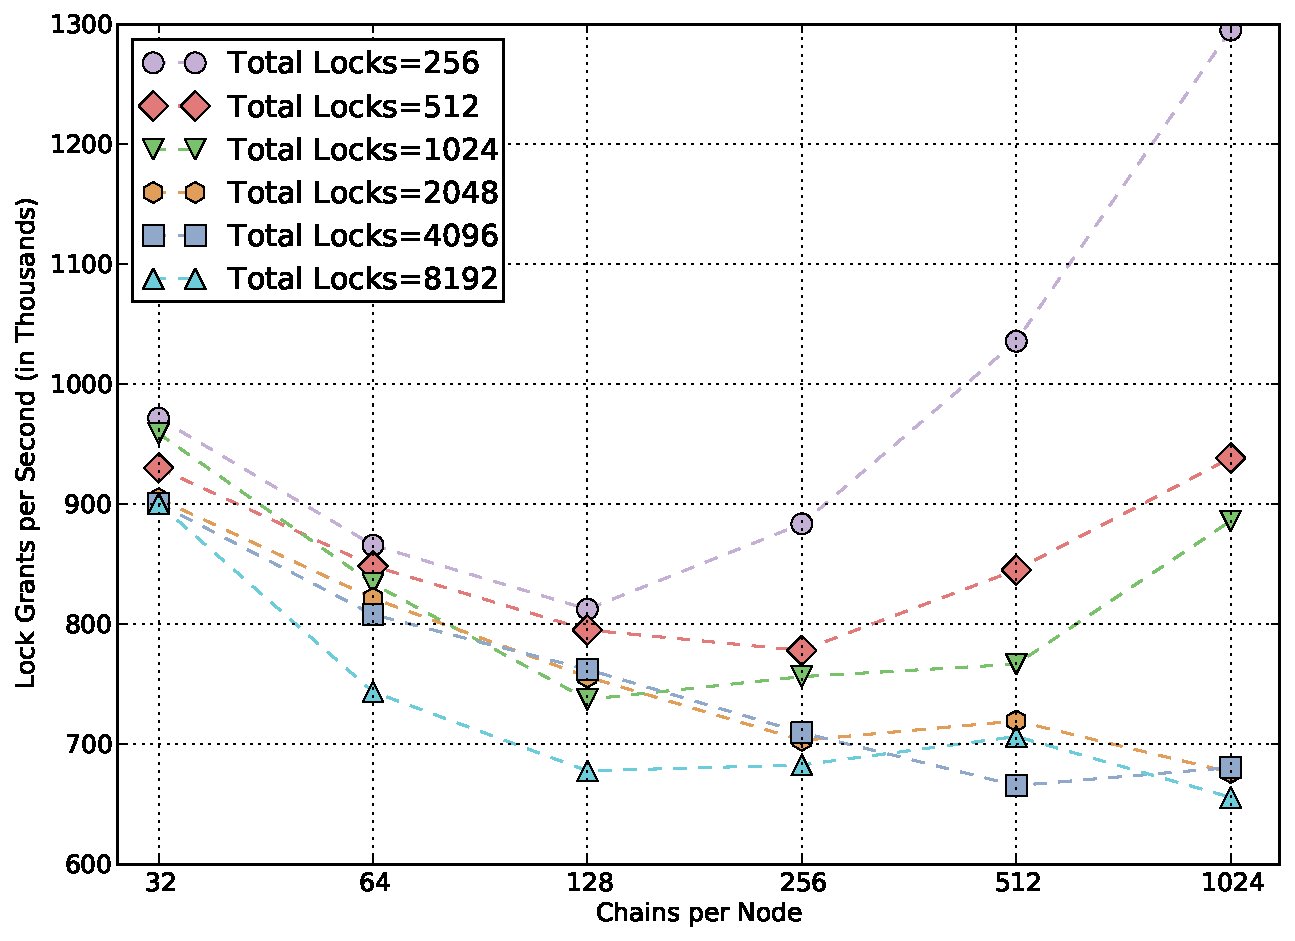
\includegraphics[scale=0.33]{figs/fixed_node_lock.pdf}
\end{center}
\vspace{-6mm}
\caption{Lock Benchmark for Fixed Node Count.\label{fig:fixednode}}
\vspace{-4mm}
\end{figure}


\subsection{Reduction Throughput}
\label{subsec:reducmicro}
To show the benefits of associating reduction operations with physical regions we designed
a histogram micro-benchmark that requires all nodes to perform an addition reduction to a
physical region located in the globally visible GASNet memory (described in 
Section~\ref{sec:impl}).  Using the reduction interface described in Section~\ref{subsec:phyreg}
reductions are performed in five ways:

\begin{itemize} \itemsep1pt \parskip0pt \parsep0pt
\item Single Reads/Writes - Each node takes a lock on the global physical region and then for each reduction
reads a values from the physical region, performs the reduction, and then write the result back.  The lock is then released.
\item Single Reductions - The reduction operation implementation performs each reduction individually
using an underlying active message implementation.
\item Localized Instance - Each node takes a lock on the the global physical region, copies it to a local physical
region, performs reductions to the localized region, copies the region back, and releases the lock.
\item Fold Instance - Each node creates a local reduction instance that folds reductions to the same element.
Reductions are applied locally and then the local reduction instance is merged back into the global region.
\item List Instance - Each node creates a local reduction instance that stores a list of reduction operations.
Reductions are applied locally and then the local reduction instance is merged back into the global region.
\end{itemize}

We run two experiments, one corresponding with dense reductions and one corresponding with sparse
reductions.  Each experiment runs 8 reduction tasks per node, one for each processor.  The dense
case has 256K buckets and each reduction task performs 4M reductions to random locations.  The results for the
dense experiment are shown in Figure~\ref{fig:reducdense}.  The sparse case has 4M buckets and
each reduction task performs 64K reductions to random locations.  Results for the sparse case
be seen in Figure~\ref{fig:reducsparse}.

The dense experiment demonstrates that using folding reduction regions perform 
best and scale with the number of nodes, achieving over a billion reductions
per second in the 16 node case.  List regions also scale, but perform about an
order of mangitude worse than folding regions in the dense case.  Not surprisingly
the other algorithms all have bottlenecks that result in poor performance.  The
sparse case is very similar with additional interesting behavior that at 16 nodes
the list regions begins performing better than the fold regions.  This shows that
list regions are better suited for scaling sparse reduction operations.

\begin{figure}
\begin{center}
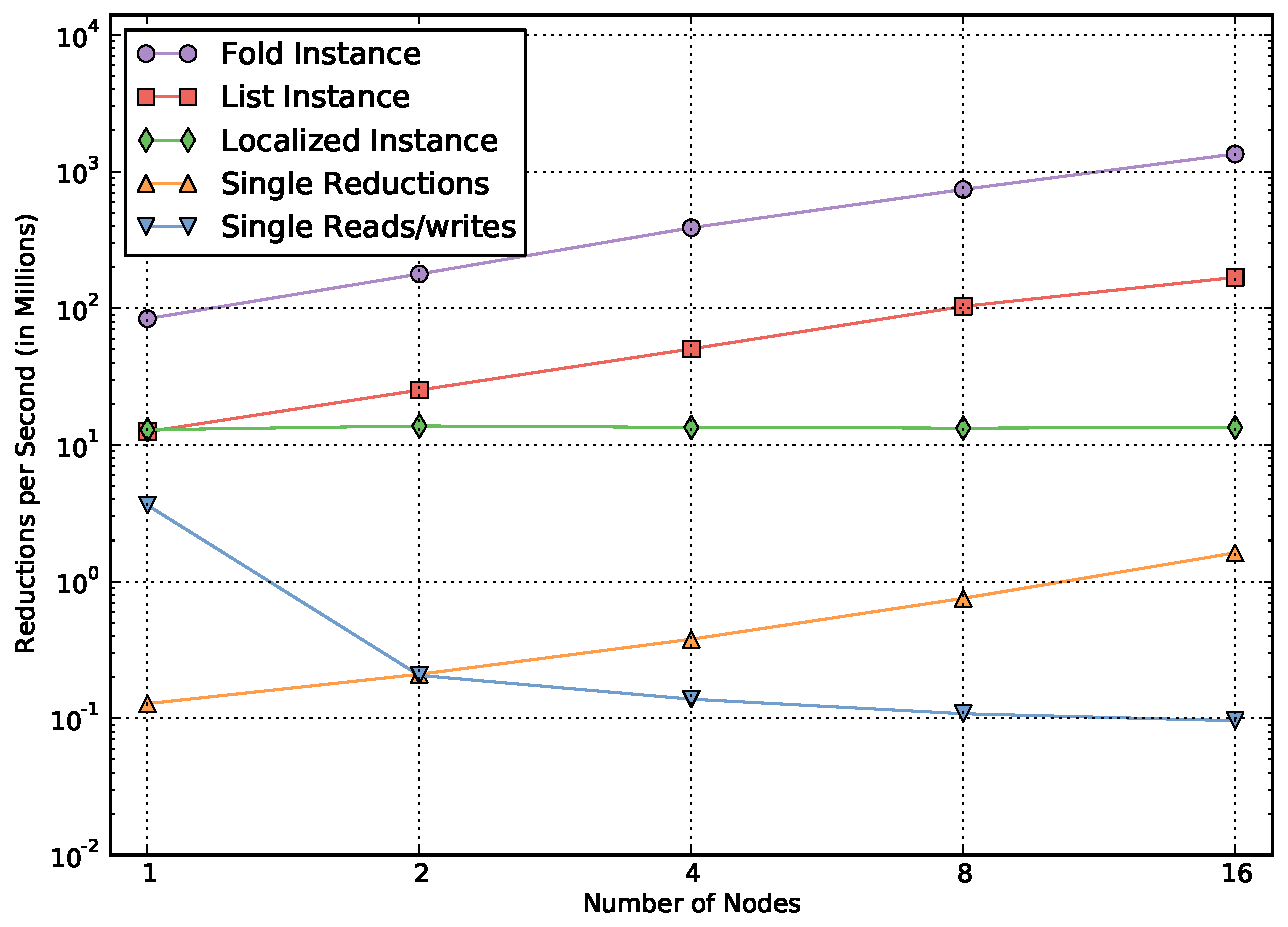
\includegraphics[scale=0.33]{figs/reduce_dense.pdf}
\end{center}
\vspace{-6mm}
\caption{Dense Reduction Benchmark.\label{fig:reducdense}}
\vspace{-4mm}
\end{figure}

\begin{figure}
\begin{center}
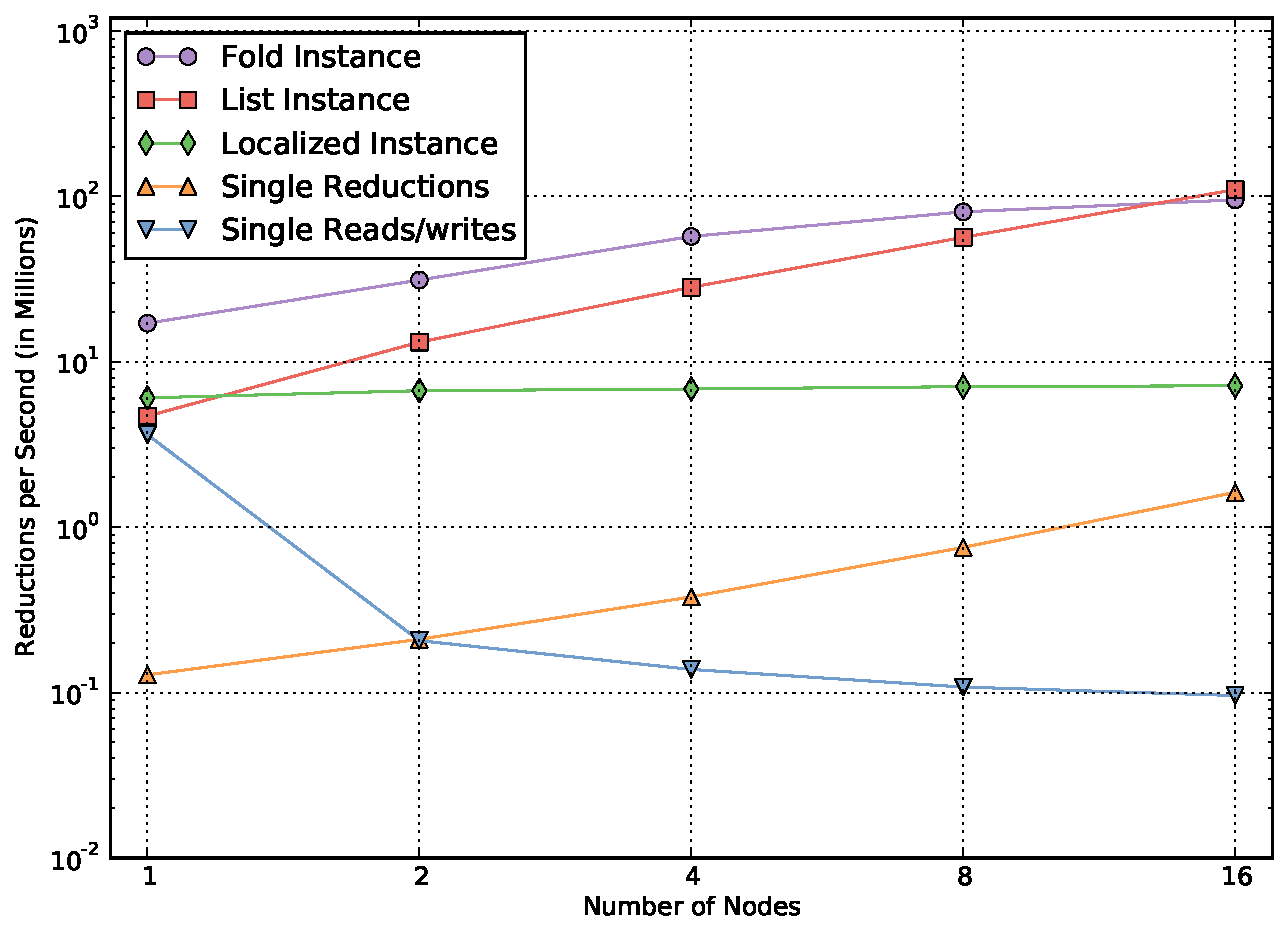
\includegraphics[scale=0.33]{figs/reduce_sparse.pdf}
\end{center}
\vspace{-6mm}
\caption{Sparse Reduction Benchmark.\label{fig:reducsparse}}
\vspace{-4mm}
\end{figure}

